\newcommand{\teaserimheight}{1.5cm}
\newcommand{\teasertextwidth}{1.5cm}
\newcommand{\teasertext}[1]{
    \begin{minipage}[b][\teaserimheight][c]{\teasertextwidth}
    \tiny
    \centering
    #1
    \end{minipage}
}
\setlength{\fboxsep}{0pt}
\setlength{\fboxrule}{0.5pt}
\newcommand{\teaserhspace}{\hspace{0.15cm}}
\newcommand{\teaserarrow}{\begin{teaserarrowbox} \centering $\longrightarrow$ \end{teaserarrowbox}}


\definecolor{llgray}{RGB}{243,243,243}
\definecolor{llpink}{RGB}{255,226,226}

\newtcolorbox{teaserpromptbox}{
    enhanced,
    boxsep=2pt,left=0pt,right=0pt,top=0pt,bottom=0pt,
    width=0.77\textwidth,
    colback={llgray},
    baseline=3.5mm,
    box align=center,
    boxrule=0.5pt,
    nobeforeafter
}
\newtcolorbox{teaseroutputbox}{
    enhanced,
    boxsep=2pt,left=0pt,right=0pt,top=0pt,bottom=0pt,
    width=0.17\textwidth,
    colback={llpink},
    baseline=3.5mm,
    box align=center,
    boxrule=0.5pt,
    nobeforeafter
}
\newtcolorbox{teaserarrowbox}{
    enhanced,
    boxsep=2pt,left=0pt,right=0pt,top=0pt,bottom=0pt,
    width=0.04\textwidth,
    colback={white},
    colbacklower=white,
    colframe=white,
    baseline=3.5mm,
    box align=center,
    boxrule=0pt,
    frame hidden,
    nobeforeafter
}



\newcommand{\teaserdialogueimheight}{3cm}
\newcommand{\teaserdialogueboxrule}{0pt}

\newtcolorbox{teaserdialogueenvelope}{
    enhanced,
    boxsep=6pt,left=0pt,right=0pt,top=0pt,bottom=0pt,
    width=\textwidth,
    colback=white,
    colframe=black,
    baseline=0mm,
    boxrule=0.85pt,
    box align=center,
    nobeforeafter
}
\newtcolorbox{teaserdialogueuserbox}{
    enhanced,
    boxsep=4pt,left=0pt,right=0pt,top=0pt,bottom=0pt,
    hbox,
    colback={llgray},
    baseline=0mm,
    boxrule=\teaserdialogueboxrule,
    frame hidden,
    nobeforeafter
}
\newtcolorbox{teaserdialogueuserboxwrap}{
    enhanced,
    boxsep=4pt,left=0pt,right=0pt,top=0pt,bottom=0pt,
    width=0.75\textwidth,
    colback={llgray},
    baseline=0mm,
    boxrule=\teaserdialogueboxrule,
    frame hidden,
    nobeforeafter
}
\newtcolorbox{teaserdialogueflamingobox}{
    enhanced,
    boxsep=4pt,left=0pt,right=0pt,top=0pt,bottom=0pt,
    hbox,
    colback={llpink},
    baseline=0mm,
    boxrule=\teaserdialogueboxrule,
    frame hidden,
    nobeforeafter
}
\newtcolorbox{teaserdialogueflamingoboxwrap}{
    enhanced,
    boxsep=4pt,left=0pt,right=0pt,top=0pt,bottom=0pt,
    width=0.75\textwidth,
    colback={llpink},
    baseline=0mm,
    boxrule=\teaserdialogueboxrule,
    frame hidden,
    nobeforeafter
}

\newcommand{\dialogueavatarsep}{\hspace{0.1cm}}
\newcommand{\useravatar}{
\includegraphics[height=0.6cm]{figures/PersonPaperColor.pdf}}
\newcommand{\flamingoavatar}{
\includegraphics[height=0.6cm]{figures/FlamingoPaperColor.pdf}}

\newcommand{\userchat}[1]{%
    \begin{flushright}
    \begin{teaserdialogueuserbox} #1 \end{teaserdialogueuserbox}%
    \dialogueavatarsep{}%
    \useravatar{}
    \end{flushright}%
}

\newcommand{\userchatw}[1]{%
    \begin{flushright}
    \begin{teaserdialogueuserboxwrap} #1 \end{teaserdialogueuserboxwrap}%
    \dialogueavatarsep{}%
    \useravatar{}
    \end{flushright}%
}

\newcommand{\flamingochatw}[1]{%
    \begin{flushleft}
    \flamingoavatar{}%
    \dialogueavatarsep{}%
    \begin{teaserdialogueflamingoboxwrap} #1 \end{teaserdialogueflamingoboxwrap}
    \end{flushleft}
}

\newcommand{\flamingochat}[1]{%
    \begin{flushleft}
    \flamingoavatar{}%
    \dialogueavatarsep{}%
    \begin{teaserdialogueflamingobox} #1 \end{teaserdialogueflamingobox}
    \end{flushleft}
}

\definecolor{shadecolor}{rgb}{0.97, 0.97, 0.97}
\newcommand{\chatsep}{\vspace{-0.35cm}}

\begin{figure}
\centering
\vspace{-0.6cm}


\begin{teaserpromptbox} \centering Input Prompt \end{teaserpromptbox}
\begin{teaserarrowbox} {$\phantom{\longrightarrow}$} \end{teaserarrowbox}
\begin{teaseroutputbox} \centering \small \flamingoemojiavatar{} Completion \end{teaseroutputbox}
\\

\begin{teaserpromptbox} \centering
    \fbox{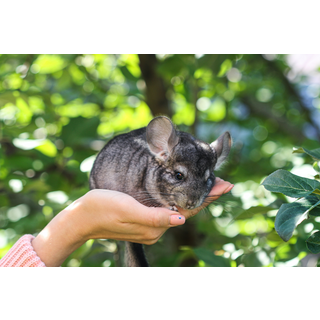
\includegraphics[height=\teaserimheight]{figures/teaserpics/teaser1a.png}}
    \teasertext{This is a chinchilla. They are mainly found in Chile.}
    \teaserhspace{}
    \fbox{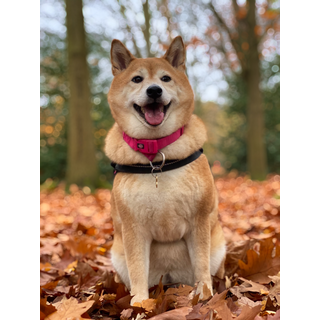
\includegraphics[height=\teaserimheight]{figures/teaserpics/teaser1b.png}}
    \teasertext{This is a shiba. They are very popular in Japan.}
    \teaserhspace{}
    \fbox{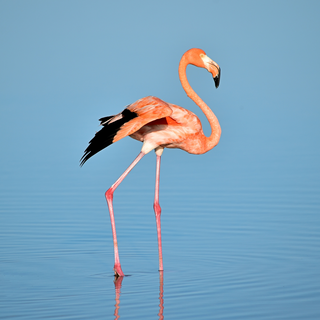
\includegraphics[height=\teaserimheight]{figures/teaserpics/teaser1c.png}}
    \teasertext{This is}
\end{teaserpromptbox}
\teaserarrow{}
\begin{teaseroutputbox} \centering \bf
    \teasertext{a flamingo. They are found in the Caribbean and South America.}
\end{teaseroutputbox}
\\

\begin{teaserpromptbox} \centering
    \fbox{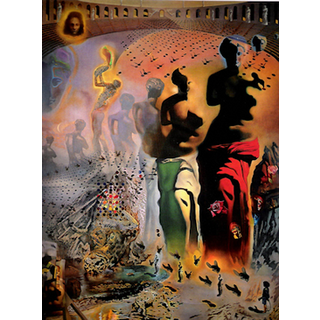
\includegraphics[height=\teaserimheight]{figures/teaserpics/teaser2a.png}}
    \teasertext{What is the title of this painting? Answer: The Hallucinogenic Toreador.}
    \teaserhspace{}
    \fbox{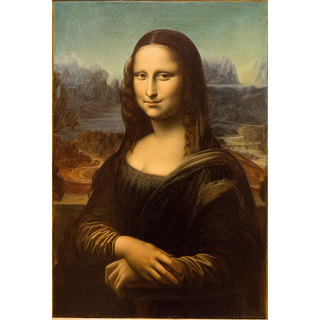
\includegraphics[height=\teaserimheight]{figures/teaserpics/teaser2b.png}}
    \teasertext{Where is this painting displayed? Answer: Louvres Museum, Paris.}
    \teaserhspace{}
    \fbox{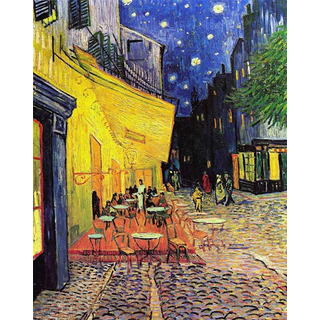
\includegraphics[height=\teaserimheight]{figures/teaserpics/teaser2c.png}}
    \teasertext{What is the name of the city where this was painted? Answer:}
\end{teaserpromptbox}
\teaserarrow{}
\begin{teaseroutputbox} \centering \bf
    \teasertext{Arles.}
\end{teaseroutputbox}
\\

\begin{teaserpromptbox} \centering
    \fbox{
\includegraphics[height=\teaserimheight]{figures/teaserpics/teaser3a.png}}
    \teasertext{Output: "Underground"}
    \teaserhspace{}
    \fbox{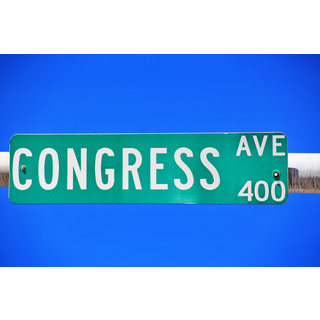
\includegraphics[height=\teaserimheight]{figures/teaserpics/teaser3b.png}}
    \teasertext{Output: "Congress"}
    \teaserhspace{}
    \fbox{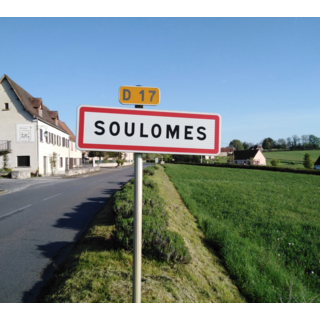
\includegraphics[height=\teaserimheight]{figures/teaserpics/teaser3c.png}}
    \teasertext{Output:}
\end{teaserpromptbox}
\teaserarrow{}
\begin{teaseroutputbox} \centering \bf
    \teasertext{"Soulomes"}
\end{teaseroutputbox}
\\

\begin{teaserpromptbox} \centering
    \fbox{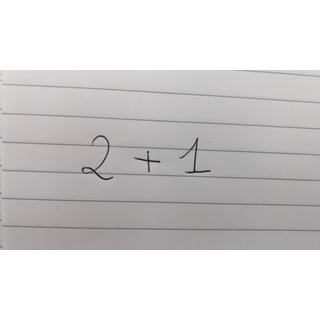
\includegraphics[height=\teaserimheight]{figures/teaserpics/teaser4a.png}}
    \teasertext{2+1=3}
    \teaserhspace{}
    \fbox{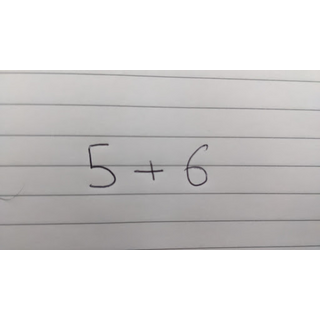
\includegraphics[height=\teaserimheight]{figures/teaserpics/teaser4b.png}}
    \teasertext{5+6=11}
    \teaserhspace{}
    \fbox{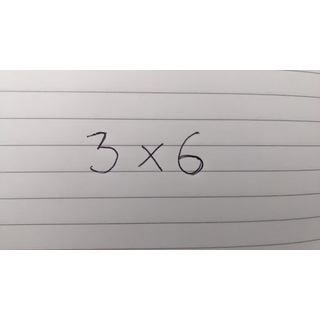
\includegraphics[height=\teaserimheight]{figures/teaserpics/teaser4c.png}}
    \teasertext{\phantom{?}}
\end{teaserpromptbox}
\teaserarrow{}
\begin{teaseroutputbox} \centering \bf
    \teasertext{3x6=18}
\end{teaseroutputbox}
\\

\begin{teaserpromptbox} \centering
    \fbox{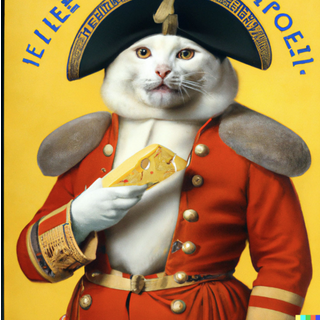
\includegraphics[height=\teaserimheight]{figures/teaserpics/teaser5a.png}}
    \teasertext{Output: A propaganda poster depicting a cat dressed as French emperor Napoleon holding a piece of cheese.}
    \teaserhspace{}
    \fbox{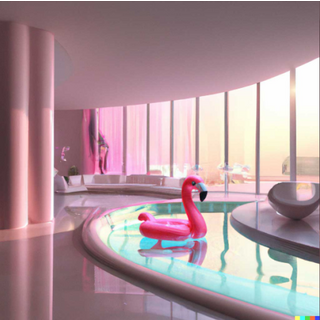
\includegraphics[height=\teaserimheight]{figures/teaserpics/teaser5b.png}}
    \teasertext{Output: A pink room with a flamingo pool float.}
    \teaserhspace{}
    \fbox{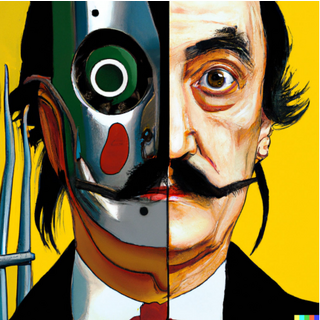
\includegraphics[height=\teaserimheight]{figures/teaserpics/teaser5c.png}}
    \teasertext{Output:}
\end{teaserpromptbox}
\teaserarrow{}
\begin{teaseroutputbox} \centering \bf
    \teasertext{A portrait of Salvador Dali with a robot head.}
\end{teaseroutputbox}
\\

\begin{teaserpromptbox} \centering
    \fbox{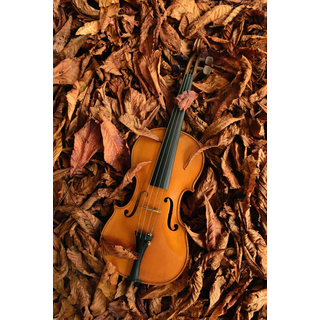
\includegraphics[height=\teaserimheight]{figures/teaserpics/teaser6a.png}}
    \teasertext{Les sanglots longs des violons de l’automne blessent mon coeur d’une langueur monotone.}
    \teaserhspace{}
    \fbox{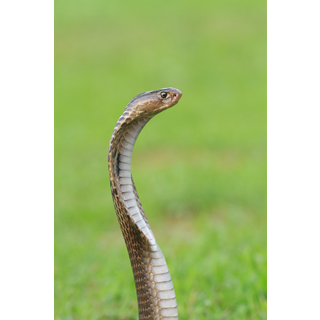
\includegraphics[height=\teaserimheight]{figures/teaserpics/teaser6b.png}}
    \teasertext{Pour qui sont ces serpents qui sifflent sur vos têtes?}
    \teaserhspace{}
    \fbox{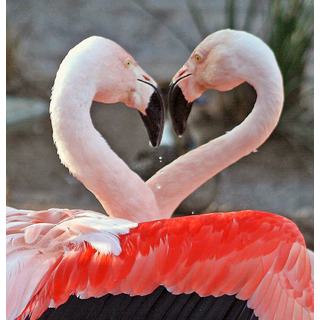
\includegraphics[height=\teaserimheight]{figures/teaserpics/teaser6c.png}}
    \teasertext{\phantom{?}}
\end{teaserpromptbox}
\teaserarrow{}
\begin{teaseroutputbox} \centering \bf
    \teasertext{Je suis un cœur qui bat pour vous.}
\end{teaseroutputbox}
\\

\begin{teaserpromptbox} \centering
    \fbox{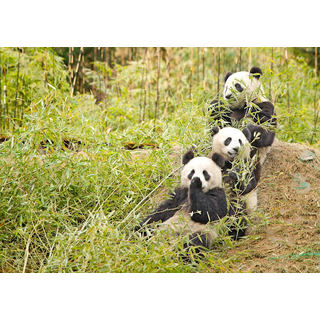
\includegraphics[height=\teaserimheight]{figures/teaserpics/teaser7a.png}}
    \teasertext{pandas: 3}
    \teaserhspace{}
    \fbox{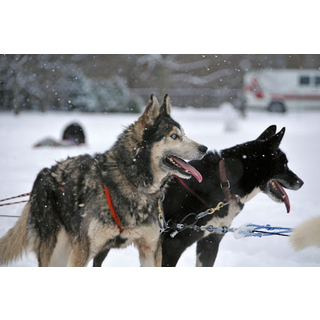
\includegraphics[height=\teaserimheight]{figures/teaserpics/teaser7b.png}}
    \teasertext{dogs: 2}
    \teaserhspace{}
    \fbox{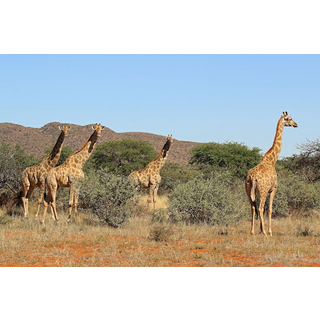
\includegraphics[height=\teaserimheight]{figures/teaserpics/teaser7c.png}}
    \teasertext{\phantom{?}}
\end{teaserpromptbox}
\teaserarrow{}
\begin{teaseroutputbox} \centering \bf
    \teasertext{giraffes: 4}
\end{teaseroutputbox}
\\

\begin{teaserpromptbox} \centering
    
\includegraphics[height=\teaserimheight]{figures/teaserpics/placeholder.png}
    \teasertext{I like reading}
    \teaserhspace{}
    \fbox{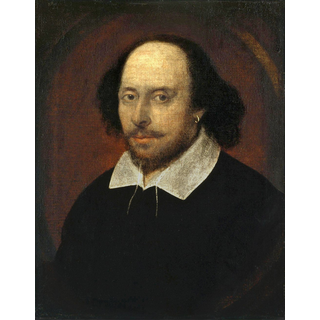
\includegraphics[height=\teaserimheight]{figures/teaserpics/shakespeare.png}}
    \teasertext{, my favourite play is Hamlet. I also like}
    \teaserhspace{}
    \fbox{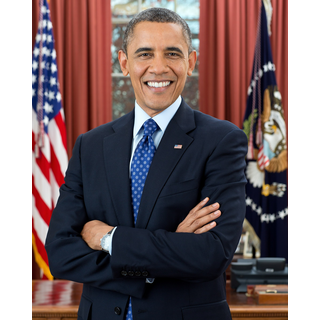
\includegraphics[height=\teaserimheight]{figures/teaserpics/obama.png}}
    \teasertext{, my favorite book is}
\end{teaserpromptbox}
\teaserarrow{}
\begin{teaseroutputbox} \centering \bf
    \teasertext{Dreams from my Father.}
\end{teaseroutputbox}
\\


\newcommand{\whitebox}{\hfill\textcolor{white}{\rule[0.46875mm]{0.84375mm}{1.3125mm}}\hfill}
\newcommand{\filmbox}[1]{%
    \setlength{\fboxsep}{0pt}%
    \colorbox{black}{%
        \begin{minipage}{\teaserimheight}
            \rule{0mm}{2.25mm}\whitebox\whitebox\whitebox\whitebox\whitebox%
            \whitebox\whitebox\whitebox\whitebox\null\\%
            \null\hfill\includegraphics[width=\teaserimheight]{#1}\hfill\null\\%[0.46875mm]%
            \null\whitebox\whitebox\whitebox\whitebox\whitebox%
            \whitebox\whitebox\whitebox\whitebox\null
        \end{minipage}}}


\begin{teaserpromptbox} \centering
    \fbox{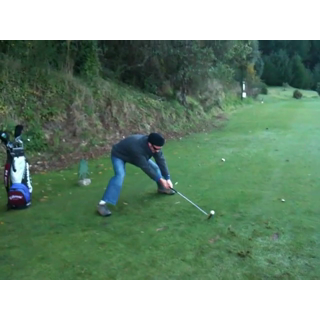
\includegraphics[height=\teaserimheight]{figures/videoframes/imvid_shot_0002.png}}
    \hspace{-0.20cm}
    \fbox{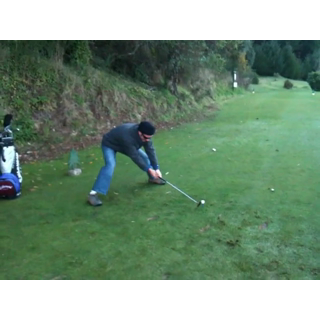
\includegraphics[height=\teaserimheight]{figures/videoframes/imvid_shot_0003.png}}
    \hspace{-0.20cm}
    \fbox{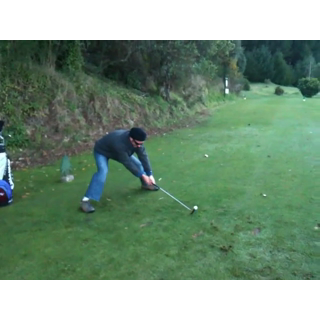
\includegraphics[height=\teaserimheight]{figures/videoframes/imvid_shot_0004.png}}
    \hspace{-0.20cm}
    \fbox{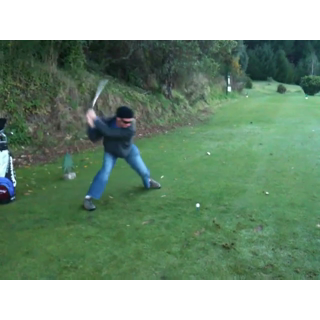
\includegraphics[height=\teaserimheight]{figures/videoframes/imvid_shot_0005.png}}
    \hspace{-0.20cm}
    \fbox{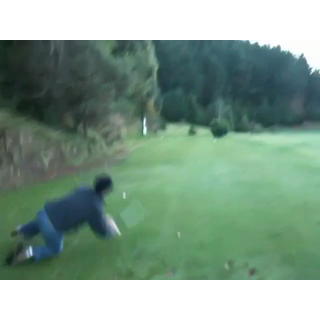
\includegraphics[height=\teaserimheight]{figures/videoframes/imvid_shot_0006.png}}
    \teasertext{What happens to the man after hitting the ball? Answer:}
\end{teaserpromptbox}
\teaserarrow{}
\begin{teaseroutputbox} \centering \bf
    \teasertext{he falls down.}
\end{teaseroutputbox}
\\


\scalebox{0.545}{
\begin{minipage}[b]{0.45\textwidth}
\begin{teaserdialogueenvelope}
\userchat{\fbox{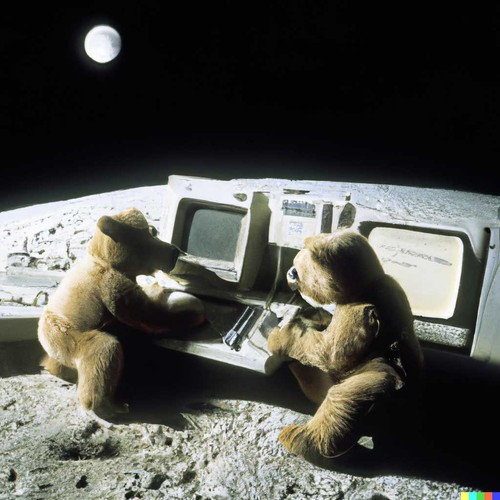
\includegraphics[height=3.2cm]{figures/moonbears.jpeg}}}
\chatsep{}
\flamingochatw{This is a picture of two teddy bears on the moon.}
\chatsep{}
\userchat{What are they doing?}
\chatsep{}
\flamingochatw{They are having a \mbox{conversation}.}
\chatsep{}
\userchat{What object are they using?}
\chatsep{}
\flamingochat{It looks like a computer.}
\chatsep{}
\userchat{Is this surprising?}
\chatsep{}
\flamingochat{Yes, it is surprising.}
\chatsep{}
\userchatw{Why is this picture surprising to you?}
\chatsep{}
\flamingochatw{I think it is surprising because teddy bears are not usually found on the moon.}
\end{teaserdialogueenvelope}
\end{minipage}
\begin{minipage}[b]{0.45\textwidth}
\begin{teaserdialogueenvelope}
\userchat{\fbox{
\includegraphics[height=1.8cm]{figures/teaserpics/flamingo_icon.png}}}
\chatsep{}
\userchat{\fbox{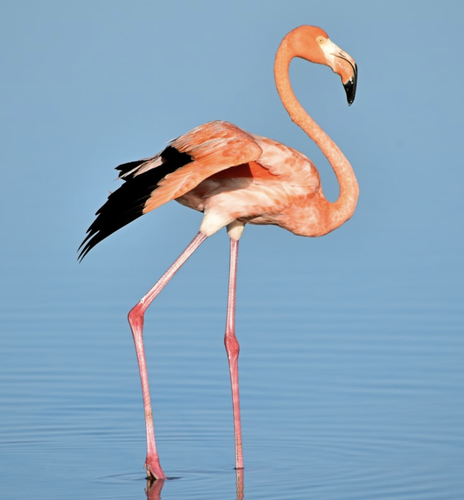
\includegraphics[height=1.8cm]{figures/teaserpics/flamingo_picture.png}}}
\chatsep{}
\userchat{\fbox{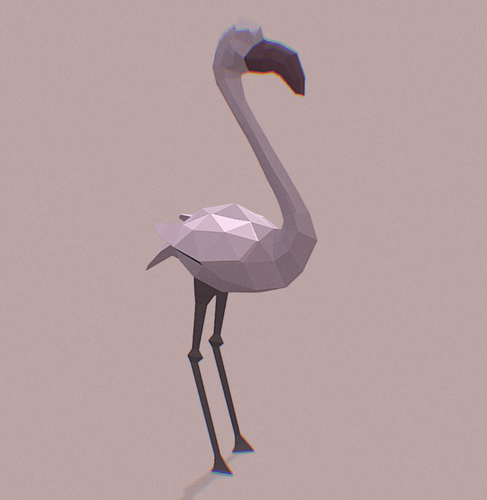
\includegraphics[height=1.8cm]{figures/teaserpics/flamingo_3d.png}}}
\chatsep{}
\userchatw{What is the common thing about \mbox{these three images?}}
\chatsep{}
\flamingochat{They are all flamingos.}
\chatsep{}
\userchatw{What is the difference between \mbox{these three images?}}
\chatsep{}
\flamingochatw{The first one is a cartoon, the second one is a real flamingo, and the third one is a 3D model of a flamingo.}
\end{teaserdialogueenvelope}
\end{minipage}
\begin{minipage}[b]{0.45\textwidth}
\begin{teaserdialogueenvelope}
\userchat{\fbox{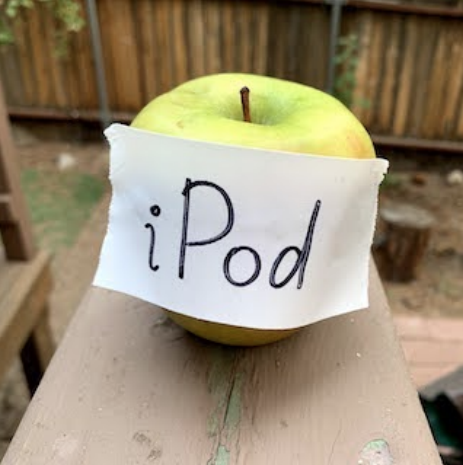
\includegraphics[height=3.8cm]{figures/appleipod.png}}}
\chatsep{}
\flamingochatw{This is an apple with a sticker on it.}
\chatsep{}
\userchat{What does the sticker say?}
\chatsep{}
\flamingochat{The sticker says "iPod".}
\chatsep{}
\userchat{Where is the photo taken?}
\chatsep{}
\flamingochatw{It looks like it's taken in a \mbox{backyard}.}
\chatsep{}
\userchatw{Do you think it is printed or \mbox{handwritten?}}
\chatsep{}
\flamingochat{It looks like it's handwritten.}
\chatsep{}
\userchat{What color is the sticker?}
\chatsep{}
\flamingochat{It's white.}
\end{teaserdialogueenvelope}
\end{minipage}
\begin{minipage}[b]{0.45\textwidth}
\begin{teaserdialogueenvelope}
\userchat{\fbox{\includegraphics[height=1.8cm]{figures/boston_skyline.png}}}
\chatsep{}
\flamingochatw{This is a cityscape. It looks like Chicago.}
\chatsep{}
\userchatw{What makes you think this is Chicago?}
\chatsep{}
\flamingochatw{I think it's Chicago because of the Shedd Aquarium in the background.}
\userchat{\fbox{\includegraphics[height=1.7cm]{figures/tokyo_skyline.png}}}
\chatsep{}
\userchatw{What about this one? Which city is this and what famous landmark helped you recognise the city?}
\chatsep{}
\flamingochatw{This is Tokyo. I think it's Tokyo because of the Tokyo Tower.}
\end{teaserdialogueenvelope}
\end{minipage}

}

\centering
\caption{\textbf{Selected examples of inputs and outputs obtained from \largemfull{}.}
\largem{} can rapidly adapt to various image/video understanding tasks with few-shot prompting (top).
Out of the box, \largem{} is also capable of multi-image visual dialogue (bottom). More examples in
Appendix~\maintoappref{app:qual_res}.
}
\label{fig:teaser}
\end{figure}